\chapter{Cycle-consistency Framework}
\label{ch:main_idea}


\graphicspath{ {./body/media/} }


%Cycle-consistency framework (main idea)
%Task formulation/formalization
%Baseline architecture -> Any seq2seq model
%Cycle architecture
%Gumbel Softmax Extension
%Semantic Similarity
%Losses used to train the models

In this Chapter, we detail our approach to automated storytelling. First, we provide a formalization of the problem (\cref{sec:formulation}). Then, we proceed to explain our baseline architecture (\cref{sec:baseline_arch}). Finally, we explain how we build on top of the baseline to get the cycle architecture and some possible extensions (\cref{sec:cycle_arch}).


\section{Problem Formulation}
\label{sec:formulation}

Previously the task of story generation has been mostly viewed as a translation task, where a model is given as input a summary/topic and is required to produce a story. A simple schema is shown in Figure \ref{fig:classical_problem_formulation}. More formally, given a conditional sequence $\mathbf{x} = (x_1, x_2, \ldots, x_{|\mathbf{x}|})$, that indicates a title, a topic or a short summary, the model is required to translate it into a sequence $\mathbf{y} = (y_1, y_2, \ldots, y_{|\mathbf{y}|})$ indicating a story that follows some constraints.

\begin{figure}[ht]
\centering
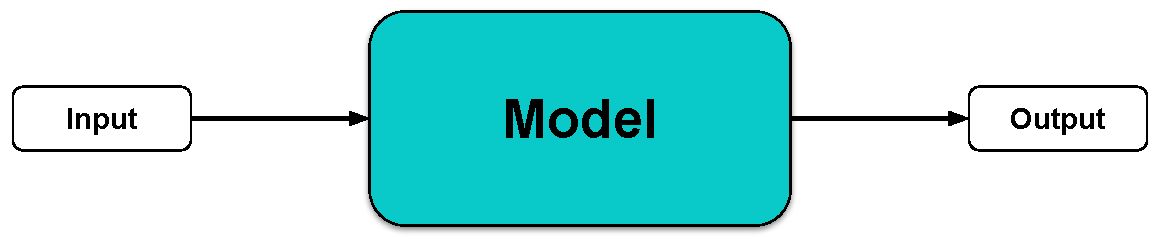
\includegraphics[width=0.75\textwidth]{classical_problem_formulation.pdf}
\caption{Traditional formulation for the story generation task}
\label{fig:classical_problem_formulation}
\end{figure}

In our work instead, we re-formulate the problem in the light of the cycle-consistency framework as shown in \cref{fig:new_problem_formulation}. To this end, given a conditional sequence $\mathbf{x} = (x_1, x_2, \ldots, x_{|\mathbf{x}|})$, a model is first required to translate it into an intermediate sequence $\mathbf{y} = (y_1, y_2, \ldots, y_{|\mathbf{y}|})$ and then another model translates $\mathbf{y}$ into an output (reconstructed) sequence $\hat{\mathbf{x}} = (\hat{x}_1, \hat{x}_2, \ldots, \hat{x}_{|\mathbf{\hat{\mathbf{x}}}|})$. The goal for $\mathbf{x}$ and $\hat{\mathbf{x}}$ is to be as close as possible.

\begin{figure}[ht]
\centering
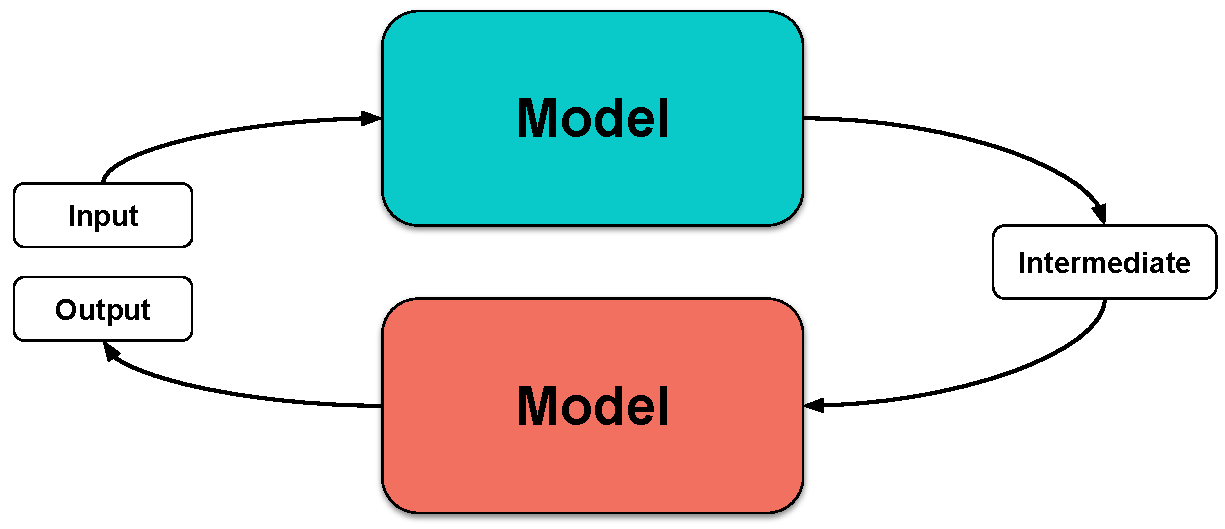
\includegraphics[width=0.75\textwidth]{new_problem_formulation.pdf}
\caption{New formulation for the story generation task}
\label{fig:new_problem_formulation}
\end{figure}

Forcing the original input and its associated reconstruction to be as close as possible leads the models to work together for achieving optimal performance. Indeed, the first model produces text that satisfies a certain task and also conveys the critical information for the other model to operate. The second model instead uses the critical signals in the intermediate text to accurately reconstruct the input. 

Our proposed framework is general enough to consider any two tasks that are considered duals (e.g., translation and back-translation). In this thesis, we specifically study text generation (expansion) and summarization (compression) applied to stories. The expanded text represents a story built from a number of sentences, while the compressed text can be a summary of the story or a title highlighting the theme.


% =================================================================================================

\section{Baseline Architecture}
\label{sec:baseline_arch}

%Since our main task of consideration is story generation, the baseline can be any seq2seq architecture like most of the previous work (\cref{ch:related_work}). However, we base our implementation on BART \citep{lewis2019bart} which is a Transformer-based seq2seq architecture. BART is an encoder-decoder architecture which makes it suitable for text generation tasks since it can both utilize the encoder to access all the input tokens and use the decoder for left-to-right generation. To obtain a baseline to use for future comparison we use one BART model for the expansion task (summary $\mapsto$ story).

Since our main task of consideration is story generation, the baseline can be any seq2seq architecture like most of previous work (\cref{ch:related_work}). The task is then formalized as a conditional generation task (see \cref{fig:baseline_model}) where we want to maximize the output probability distribution
\[ p(\mathbf{y} \mid \mathbf{x}) = \prod_{i=1}^{|\mathbf{y}|} p(y_i \mid \mathbf{y}_{<i}, \mathbf{x})  \]
where $\mathbf{x}$ is the conditional input sequence (summary) and $\mathbf{y}$ is the output sequence (story).

We use BART \citep{lewis2019bart} as our baseline architecture (discussed in \cref{sec:bart_intro}). Using BART gives us the advantage of using the massive knowledge gained from the corpora used to pretrain the model.

\begin{figure}[ht]
\centering
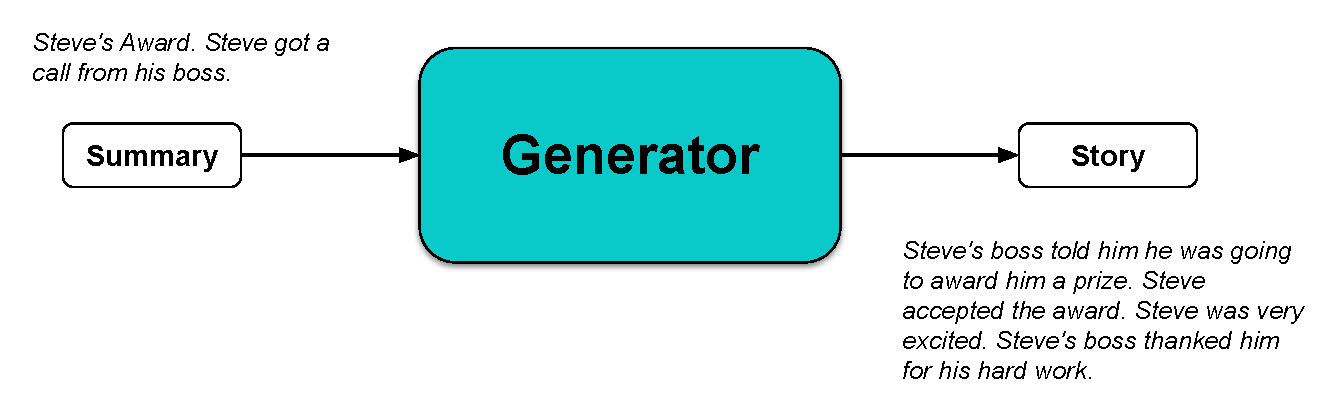
\includegraphics[width=0.75\textwidth]{baseline_model.pdf}
\caption{Baseline seq2seq model}
\label{fig:baseline_model}
\end{figure}


% =================================================================================================

\section{Cycle Architecture}
\label{sec:cycle_arch}

The key concept in this architecture is simplicity. We simply augment the baseline architecture (\cref{sec:baseline_arch}) with another seq2seq model, connect them and let them interact.

The first model performs a conditional generation task where it takes an input sequence $\mathbf{x}$ and maximizes a probability distribution $p(\mathbf{y} \mid \mathbf{x})$ for an intermediate sequence $\mathbf{y}$
\[ p(\mathbf{y} \mid \mathbf{x}) = \prod_{i=1}^{|\mathbf{y}|} p(y_i \mid \mathbf{y}_{<i}, \mathbf{x})  \]

Then the second model samples its input $\mathbf{y}$ from the intermediate probability distribution $\mathbf{y} \sim p(\mathbf{y} \mid \mathbf{x})$ and in turn maximizes a probability distribution $p(\hat{\mathbf{x}} \mid \mathbf{y})$ for an output sequence $\hat{\mathbf{x}}$
\[ p(\hat{\mathbf{x}} \mid \mathbf{y}) = \prod_{i=1}^{|\hat{\mathbf{x}}|} p(\hat{x}_i \mid \hat{\mathbf{x}}_{<i}, \mathbf{y})  \]

Similar to the baseline, we use BART as our architecture for both models. How to sample the intermediate sequence $\mathbf{y}$ from the probability distribution is discussed in the next section (\cref{sec:gumbel_softmax}).

Due to the cyclic nature of the framework, we can set $\mathbf{x}$ and $\hat{\mathbf{x}}$ to be the original and reconstructed summaries respectively, and set $\mathbf{y}$ to the generated story (see \cref{fig:cycle_model_direction_comp}); and also vice versa where $\mathbf{x}$ and $\hat{\mathbf{x}}$ are the original and reconstructed stories respectively, and $\mathbf{y}$ to the generated summary (see \cref{fig:cycle_model_direction_exp}).

\begin{figure}[ht]
    \centering
    \begin{subfigure}[b]{\textwidth}
        \centering
       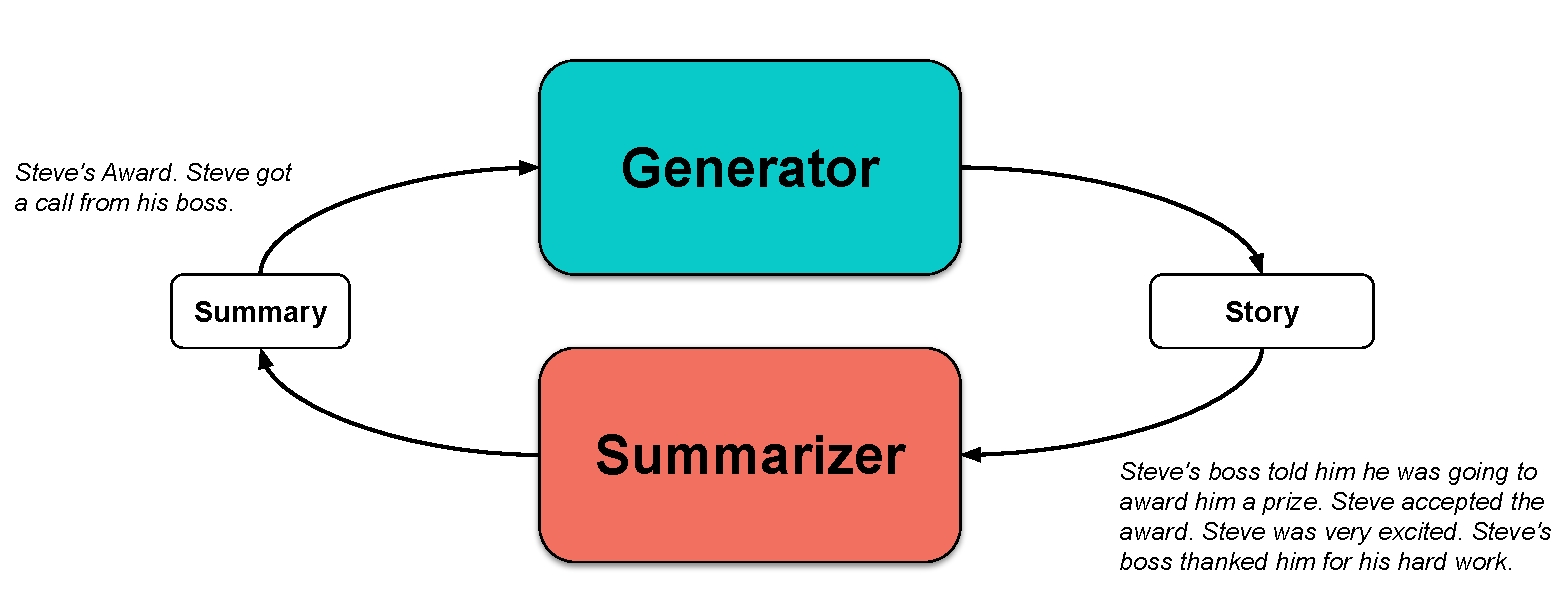
\includegraphics[width=0.75\textwidth]{cycle_model_direction_comp.pdf}
        \caption{First direction: Summary $\rightarrow$ Story $\rightarrow$ Summary}
        \label{fig:cycle_model_direction_comp}
    \end{subfigure}
    \newline \newline
    \begin{subfigure}[b]{\textwidth}
        \centering
       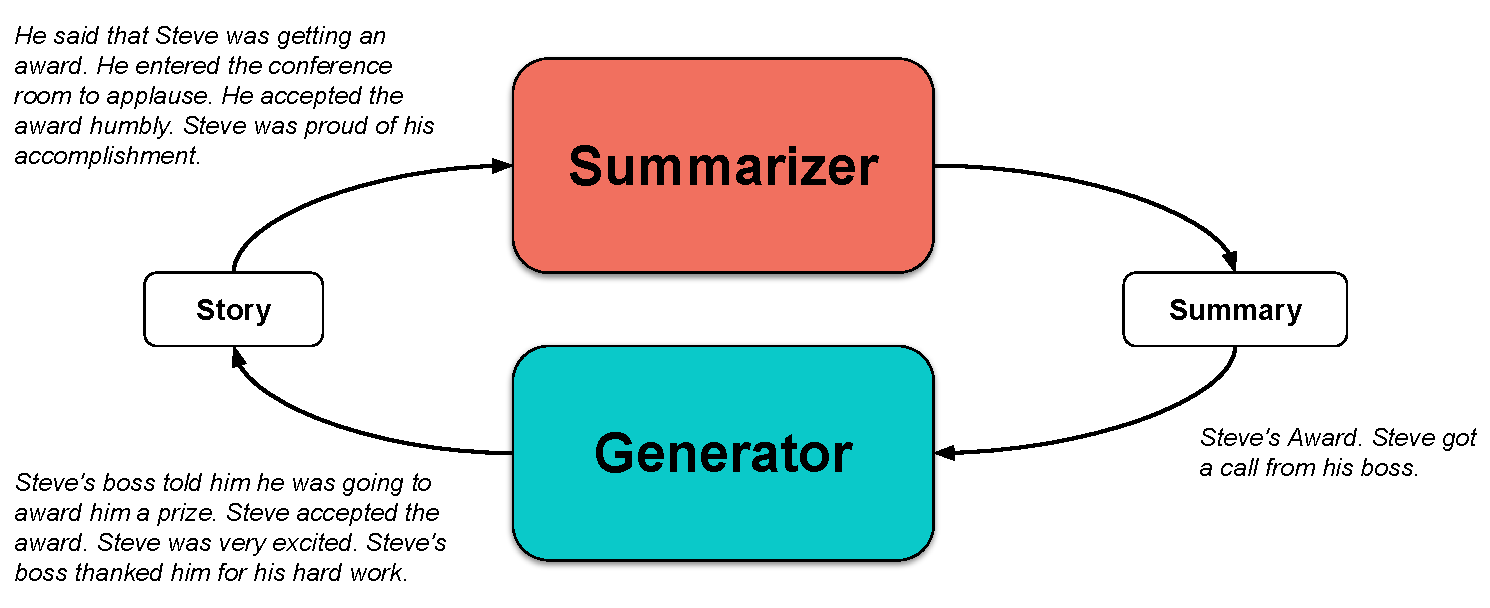
\includegraphics[width=0.75\textwidth]{cycle_model_direction_exp.pdf}
        \caption{Second direction: Story $\rightarrow$ Summary $\rightarrow$ Story}
        \label{fig:cycle_model_direction_exp}
    \end{subfigure}
    \caption{Cyclic nature of the framework}
    \label{fig:cycle_directions}
\end{figure}

An immediate observation from our proposal is the possibility to obtain two good-performing models instead of one; one performs well in expansion (generation), while the other performs well in compression (summarization). However, we only analyze the effect on the expansion process and leave the compression for another study.


% =================================================================================================

\section{Differentiable Sampling}
\label{sec:gumbel_softmax}

To generate the intermediate sequence $\mathbf{y}$, we need to sample the words $(y_1, y_2, \ldots, y_{|\mathbf{y}|})$ from the first model's output categorical distribution: 
\[ p(y_t \mid \mathbf{y}_{<t}, \mathbf{x}) = \text{softmax}(v_t) \]
where $v$ is the unnormalized output (logits) of the model. The simplest method to do so is to use greedy decoding where at each time step $t$ we look for the token with the highest probability:
\[ y_t = \text{argmax} \; p(y \mid \mathbf{y}_{<t}, \mathbf{x}) \]

Since this process uses the argmax operation it is non-differentiable. This results in a training mode similar to \citep{he2016dual} where each model trains separately and they are related only by any information passed through the intermediate text.

To retain the ability to train the whole model using gradient-based optimization where the gradients can backpropagate through both models, we use the Gumbel-softmax (GS) reparameterization trick as an approximation of sampling from categorical distributions \citep{jang2016categorical}. Sampling from the softmax distribution is equivalent to adding to each logit an independent noise factor $\zeta$ from the Gumbel distribution G(0, 1) ($\zeta = -\log(-\log(x_i)), \; x_i \sim Uniform(0, 1) $), and then applying the argmax operation:
\[ y_t \sim \text{softmax}(v_t) \quad \equiv \quad y_t = \text{argmax}(v_t + \zeta) \]

Next, we follow \citep{goyal2017differentiable} in using a soft approximation of the argmax using a peaked softmax function:
\[ e_t = \sum_{i}^{|V|} e(w_i) \; \text{softmax}((v_t + \zeta) / \tau ) \]
where the input for each time step is a weighted sum of all the vocabulary's embeddings and $\tau \in [0, \infty[$ is the temperature used to control the softmax. As $\tau \rightarrow \infty$, the equation approaches a true argmax embedding. Therefore, for a finitely large $\tau$, the obtained embedding is a continuous function of a linear combination of all the embeddings dominated by the most probable word.

By combining the Gumbel-softmax reparameterization trick with the soft argmax, we obtain embeddings that are continuous (thus, differentiable), and maintain the ability to sample from a distribution that adds randomness to make the model robust.

\subsubsection{Straight-Through Estimator}

In our application, we are constrained to sample discrete values (words) from the distribution. As a result, we can not use the continuous approximation shown previously. To this end, we make use of the biased Straight-Through Estimator \citep{bengio2013estimating}. We use the argmax to discretize $\mathbf{y}$ in the forward pass, but in the backward pass, we compute the gradients using the GS soft approximation.


% =================================================================================================

%\section{Semantic Similarity}

%To improve the quality of the generated stories, we impose an extra measurement that focuses on the semantics of the story. The goal for this metric is to motivate the generated story to be as close as possible to the true story \textit{semantically}. A straightforward approach would be to compute the contextualized embeddings of the generated story and label story and maximize the cosine similarity between the vector embeddings. However, we suspect that this approach might create some bias where it forces our model to learn the contextual embedding of the label story.

%Instead our goal is to learn the similarity between the two vectors. First, we finetune a BERT model to our stories dataset. Then during training time, we feed the two stories -- generated and label --  to BERT using the built-in separator token (\texttt{[SEP]}) and use the output \texttt{[CLS]} vector to learn this similarity. We repeat the same process for $k$ negative samples and obtain $k$ \texttt{[CLS]} vectors. We feed the $k$ \texttt{[CLS]} vectors to a linear layer with a pair-wise softmax output that maximizes the score of the correct generated story.

%The semantic similarity module is trained to optimize the following TF-IDF weighted cross-entropy objective function:

%\[ \mathcal{L} = - \sum_{y}^{\mathcal{Y}} \mathcal{P}(x, y) \, \log \mathcal{F}(\{x, y\}; \theta)  \]
%\[ \mathcal{L} = - \sum_{y}^{\mathcal{Y}} \, \log \mathcal{F}(\{x, y\}; \theta)  \]
%\[ \mathcal{L} = - \sum_{i}^{N} \log \mathcal{F}(\{x, y^{+}\}; \theta) + \log(1- \mathcal{F}(\{x, y^{+}\}; \theta)) \]

%where $x$ is the label story, $\mathcal{Y} = \{y^{+}, \bigcup y^{-} \}$ is the set of the generated story and all the negative samples, $\mathcal{F}$ is the probability output of the softmax described above, and $\mathcal{P}$ is a TF-IDF weighting term which calculates the distance between two constructed vectors of the label story and sample story. The constructed vector is a TF-IDF weighted sum of the word embeddings of the story.

%\[ \mathcal{P}(x, y) =  \left\lVert \sum_{i=1}^{N} \frac{\text{IDF}(x_i)}{\sum_{t=1}^{N} \text{IDF}(x_t)} \, e_{i}^{x} \;-\; \sum_{i=1}^{M} \frac{\text{IDF}(y_i)}{\sum_{t=1}^{M} \text{IDF}(y_t)} \, e_{i}^{y} \right\rVert \]

